\documentclass[pldi,10pt,preprint]{sigplanconf-pldi16}

% The following \documentclass options may be useful:

% preprint      Remove this option only once the paper is in final form.
% 10pt          To set in 10-point type instead of 9-point.
% 11pt          To set in 11-point type instead of 9-point.
% authoryear    To obtain author/year citation style instead of numeric.

\usepackage{graphicx}
\usepackage{caption}
\usepackage{subcaption}

\begin{document}

% \newcommand{\charcoal}{Charcoal}
\newcommand{\charcoal}{BlindReview}

\special{papersize=8.5in,11in}
\setlength{\pdfpageheight}{\paperheight}
\setlength{\pdfpagewidth}{\paperwidth}

\conferenceinfo{CONF 'yy}{Month d--d, 20yy, City, ST, Country}
\copyrightyear{2014}
\copyrightdata{978-1-nnnn-nnnn-n/yy/mm}
% \doi{nnnnnnn.nnnnnnn}

\titlebanner{Preprint.  Please do not redistribute}        % These are ignored unless
\preprintfooter{Preprint.  Please do not redistribute}   % 'preprint' option specified.

\title{Pseudo-Preemptive Threads: A New Multitasking Primitive for Reliable, Composable and Maintainable Software}
\subtitle{Why Events, Preemptive Threads and Coroutines are All Bad Ideas\footnotemark}

\authorinfo{Blind Review}
           {Blind Review University}
           {BlindReview@BlindReview.edu}
%% \authorinfo{Benjamin Ylvisaker}
%%            {Colorado College}
%%            {ben.ylvisaker@coloradocollege.edu}

\maketitle

\begin{abstract}

The need for frequent network communication and rich physical world interaction is making multitasking a larger and larger part of modern mainstream software.
Existing abstractions for multitasking (events, coroutines, threads) all have serious software engineering problems.
In this paper we introduce a new multitasking abstraction called pseudo-preemptive threads that combines the best of coroutines and threads.
This new abstraction will make it easier for regular programmers to write sophisticated multitasking applications.

This paper has a detailed comparison of pseudo-preemptive threads with established multitasking abstractions.
It also describes novel implementation techniques, like a new call frame allocation strategy and a super fast yield implementation.
Finally we report performance results for several microbenchmarks using the prototype implementation of pseudo-preemptive threads that we developed.

\end{abstract}

% \category{CR-number}{subcategory}{third-level}

% general terms are not compulsory anymore,
% you may leave them out
% \terms
% term1, term2

% \keywords
% keyword1, keyword2

\footnotetext{This tongue-in-cheek subtitle is a reference to Ousterhout \cite{Ousterhout1996} and von Behren, et al. \cite{Behren2003a}}

\section{Introduction}

Modern mainstream software is substantially more concurrent than its forebears, in the sense that frequent network communications, rich physical world interactivity, and factoring applications into communicating processes (microservices) have become common.
Note that in this paper we are mostly not concerned with concurrency in the sense of running software on multiple processors simultaneously (i.e. parallelism).
We use \emph{multitasking} to refer to the subset of concurrency that is not parallelism.

Multitasking has some intrinsic software engineering challenges: applications must somehow be capable of handling real world events happening in an order that cannot be known when the application is written.
Existing abstractions for multitasking, like events, (preemptive) threads and coroutines, compound this intrinsic challenge with problems of their own.

This paper introduces a new multitasking abstraction called \emph{pseudo-preemptive threads} (or \emph{activities}) that we claim has software engineering benefits compared to existing alternatives.

\subsection{Background}

We begin with a brief summary of the problems with existing multitasking abstractions.

\textbf{Events}.
The most serious problem with events is that only one event handler can be running at a time.
This means that long-running tasks (including tasks that must wait indefinitely for something outside the program itself) must be \emph{manually} broken up into multiple event handlers.
This makes the logical flow of the program hard to reason about, both for programmers and analysis tools.
It can also make allocation and deallocation of resources whose lifetime spans multiple handlers much trickier.
This leads to a style of programming referred to as \emph{stack ripping} \cite{Adya2002}, or more colloquially \emph{callback hell}.
These and more subtle problems are well analyzed and criticized by von Behren et al. in \cite{Behren2003a}.

\textbf{Threads}.
Threads allow programmers to write multitasking software in a more natural style than events, because the system automatically interleaves the execution of multiple tasks.
Threads also open the door to a variety of nasty concurrency defects, which in the context of \emph{events} either cannot happen or are much easier to avoid.
Fear of these defects (data races, deadlocks, atomicity violations, livelocks, starvation, order violations) has limited the use of threads in many applications and ecosystems.
One good entry into the vast literature on diagnosing and fixing multithreading defects is \cite{Lu2008}.
These challenges have been understood for a long time; two decades ago Ousterhout wrote a good analysis and critique of the problems with threads \cite{Ousterhout1996}.

\textbf{Coroutines}.
The increasingly sophisticated multitasking in mainstream software and the well-known problems with events and threads have forced language designers to explore alternatives in recent years.
The most widely used alternative is \emph{coroutines}\footnote{In many cases language designers chose to use terms other than \emph{coroutine} for reasons that we can only speculate about.}.
Examples include async/await, which was added to the C\#/.Net ecosystem in 2012; function generators, which were added to the JavaScript ecosystem with ECMAScript 6 (standard published in 2015); even the C++ community is considering adding support for coroutines (D4134, proposed for C++17).

Since widespread use of coroutines is much more recent than events and threads, there is far less published on their pitfalls.
The central awkwardness with coroutines is that programmers must \emph{manually} partition procedures (methods, functions, subroutines, whatever) into \emph{regular procedures} and coroutines.
``Calling'' a coroutine actually spawns a task that runs concurrently with the executing code.

Like threads, multiple coroutines can be in progress simultaneously.
Unlike threads, context switching between coroutines is only permitted when a \emph{yield} primitive is \emph{explicitly} invoked.
Regular procedures \emph{cannot} yield; in other words, regular procedure calls are atomic.
A somewhat non-obvious consequence of this atomicity is that coroutines spawned by regular procedures cannot start running until the procedure returns back to a coroutine (possibly through some stack of procedure calls) that can yield.

A more detailed analysis of coroutines, including comparisons with the new abstraction introduced in this paper appears in next section.
The primary problem to remember about coroutines is that choosing which procedures should be coroutines is not always easy.
This problem is compounded during maintenance, when changing a regular procedure to a coroutine (or vice versa) can introduce bugs.

\textbf{Cooperative Threads}.
Cooperative threads are syntactically similar to preemptive (i.e. normal) threads.
However, cooperative threads cannot be interrupted at any arbitrary point chosen by the system, which has profound semantic consequences.
Like coroutines, cooperative threads must \emph{explicitly} yield to permit switching.
Unlike coroutines, programmers are free to add yield invocations anywhere, which eliminates the need for a separate category of procedures.

The biggest software engineering problem with cooperative threads is that it is hard to know which procedures might yield and which will not.
In other words, which procedure calls are atomic?
The answer to this question is very important for avoiding concurrency bugs like atomicity violations, but cooperative threads make it tricky.
This atomicity issue is especially problematic during maintenance, when adding yield (or removing) a yield can have unexpected negative consequences on the possible interleavings of threads.

Cooperative threads are not as widely used as events, threads and coroutines.
We are not aware of any thorough analyses of why this is the case, but we suspect the central issue is with the problem of determining which procedure calls are atomic.

\textbf{Hybrids}.
Researchers have understood the weaknesses of existing multitasking abstractions for a while.
Many proposals have been made for event/thread hybrids; for example: \cite{Boudol2007, Boussinot2006, Cunningham2005, Dabrowski2006, Fischer2007, Kerneis2014, Krohn2007, Li2007, Behren2003}.
A detailed comparison with all of these proposals is beyond the scope of this paper.
In the related work section we highlight the differences with the ones that are most similar to ours.

\textbf{Other Multitasking Abstractions}.
This introduction does not cover multitasking abstractions exhaustively.
We described the abstractions that are most closely related to activities.
The related work section briefly describes connections with more distantly related abstractions.

\subsection{Activities}

This paper introduces a new multitasking abstraction called \emph{pseudo-preemptive threads} or \emph{activities}.
Activities are a hybrid between cooperative and preemptive threads (as the name suggests).
Among the hybrids mentioned above, activities are most similar to \cite{Boudol2007}.

The main idea is to start with cooperative threads, then add \emph{automatically inserted} yields to make activities a bit more like preemptive threads, and a scoped \emph{no-yield} primitive for overriding yields and enforcing atomicity.

The authors of \cite{Boudol2007} were primarily concerned with \emph{proving} that yields can be inserted in a way that makes unfairness (i.e. a single thread executing indefinitely) impossible.
Our proposal compromises on provable fairness, but rather focuses on simple programmer control over yielding and implementation efficiency.

After defining activities more precisely in the next section, we provide more detailed comparisons with established multitasking abstractions.
In particular, we argue that activities combine most of the software engineering strengths of the other abstractions, while eliminating or substantially mitigating their weaknesses.

To validate the ideas presented in this paper, we implemented activities in a dialect of C that we call \charcoal{}.
In particular, we focus on two efficiency issues: memory scalability and yield performance.
All thread-like abstractions have the challenge of determining how call frames should be allocated.
We introduce a new allocation strategy called \emph{hot stacking} that has extremely low memory overhead and leads to call/return performance that is almost as good as plain C.
We describe our novel yield implementation, which minimizes the performance impact of frequent yielding.
The \charcoal{} implementation and all the benchmarking code reported in this paper are available publicly on GitHub [address removed for blind review].

% We also tweaked two real-world multithreaded C programs to use activities instead of threads to explore the software engineering implications.

\subsection{Contributions}

This paper has three primary contributions:

\begin{itemize}
\item Introduction of \emph{pseudo-preemptive threads/activities}.
\item Introduction of \emph{hot stacking}.
\item A novel high-performance implementation of yield.
\end{itemize}

\section{Pseudo-Preemptive Threads}

\emph{Pseudo-preemptive threads\slash activities} can be understood as cooperative threads plus automatic yield insertion and no-yield.
The automatic yield insertion makes activities behave more like preemptive threads from an application programmer's perspective.
However, activities are still far more resistant to concurrency bugs than threads.

Before going into any more detail on the definition and implementation of activities, we consider an example stolen from \cite{Krohn2007}; a \charcoal{} version is in Figure \ref{fig:charcoal_multidns}.
This example performs \texttt{n} DNS lookups concurrently using the standard \texttt{getaddrinfo} procedure.
It has a parameter (\texttt{max\_conc}) to limit the number of DNS requests that will be sent concurrently to avoid flooding the network with too many requests.

\begin{figure}
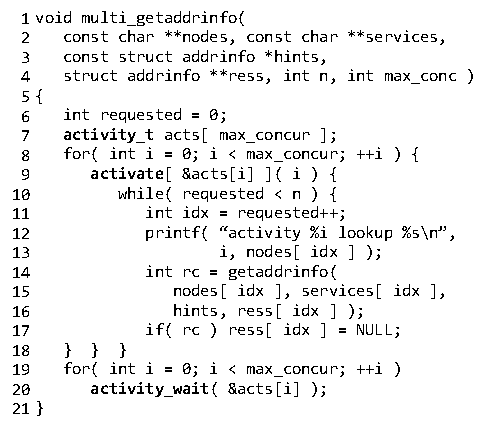
\includegraphics{multi_getaddrinfo}
\caption{A running example.
  This code concurrently performs DNS lookups.
  The maximum number of outstanding requests is \texttt{max\_conc}.}
\label{fig:charcoal_multidns}
\end{figure}

\subsection{Activate}

The central syntactic addition is the \emph{activate} statement (line 9).
The activate statement creates a new activity that runs the body of the activate statement concurrently (but not in parallel) with whatever comes after the statement (i.e. its continuation).
Only one activity can be running at a time, and the system can only context switch between activities on a yield.
By default when a program hits an activate, the body will start running before the continuation.

The semantics of a program with activities can be seen as traces of actions separated by yield invocations.
Between two adjacent yield actions, all actions must come from a single particular activity.
Batches from different activities are interleaved to execute a complete program.
Actions are not permitted to cross yield boundaries.
In other words, yields define the minimum granularity of interleaving.

The system has a scheduler that chooses when a yield should lead to a context switch, and which activity to switch to.
The current \charcoal{} implementation uses a simple FIFO scheduler; clearly this is something that could be looked at for further refinement.

The activate statement takes as a parameter a pointer to application-allocated memory for storing metadata about the new activity.
In the above example the memory for storing activity information is allocated locally.
Because of this the example procedure must wait for all the activities it spawns to finish.
(Returning before they finish could cause the program to access deallocated memory).
It would be possible to change the interface so that the caller passes in the backing memory.
In that case, the procedure could return while the activities were still fetching DNS information, allowing the application to go on with other work.
If activities were implemented in a language with automatic memory management, we would not have to be concerned about these memory allocation issues.

So far in this description, activities are identical to conventional cooperative threads.
\charcoal{} has an explicit yield statement, though it is not often needed.

\subsubsection{Local Variables}

Notice that multiple activities read and write the local variable \texttt{requested} without any additional synchronization.
If these were threads, this would cause a data race, which at best leads to unpredictable results and at worst makes the whole program undefined.
With activities this is not a problem at all; the system (compiler, processors, etc.) is not permitted to move memory operations across yields, which dramatically simplifies the concurrent memory model problem.

The parentheses after the \texttt{activate} keyword are for controlling whether local variables are accessed by-value or by-reference.
The default is by-reference, which is how most of the variables are used in this example.
The exception is \texttt{i} which is used as a name of sorts in the \texttt{printf} call.
Each activity gets its own copy of \texttt{i}, with the initial value of whatever the variable's value was at activity creation time.
If there were a modification to \texttt{i} inside \texttt{activate}, each activity would be modifying its own copy.

\subsection{Yield Insertion}

The first feature that distinguishes activities from cooperative threads is automatic yield insertion.
The goal of yield insertion is to prevent an activity from running indefinitely or waiting on an external event, and blocking other activities from making progress.
As mentioned above, the authors of \cite{Boudol2007} take this idea (fairness/starvation avoidance) to an extreme, designing a system that is provably fair.
We are less concerned with provability, and state the following as goals/guidelines rather than strict rules for activities:

\begin{enumerate}
\item It should \emph{not} be possible for an activity to run indefinitely or block without yielding.
\item Yields should happen infrequently.
\end{enumerate}

These goals are clearly in tension with each other: the first could be satisfied by yielding after every statement; the second could be satisfied by never yielding.
We do not consider it necessary to interpret these rules strictly, because we believe yield frequency bugs to be relatively easy to find an eliminate.
Profilers can easily monitor the time since the last yield and issue a warning when it has been too long.

In the example code there will be two yields inserted automatically: one at the end of the while loop that starts on line 10 and one in the implementation of \texttt{getaddrinfo} on line 14.

In general, the \charcoal{} compiler inserts a yield at the \emph{end} of every loop iteration.
Implementing this completely is somewhat tricky, because the compiler must be careful about things like continue and goto statements.
The implementation also ensures that system calls are performed in such a way that the calling activity will yield if the call might take a long time.
There are more details in the implementation section.

There is one slightly tricky concurrency bug that this example avoids in a somewhat subtle way.
The increment on line 11 must come before the call to \texttt{getaddrinfo}.
The system might context switch at that call, and its important that other activities see the incremented version of the \texttt{requested} variable.

%% These automatically-inserted yields make activities behave more like threads than events or coroutines from an application programmer's perspective.
%% However, there is a big difference between activities and threads.

%% %



%% Part of the definition of activities is that by default yields should happen ``frequently''.
%% But what does this mean precisely?
%% The answer depends on the details of the rest of the programming language definition.
%% However we can state two design rules that apply to any language.
%% These rules are in strong tension with each other:


%% One clear consequence of these rules is that anything that could cause an activity to pause indefinitely (e.g. a syscall) by default must be modified to allow other activities to run while the paused activity waits.
%% More challenging, loops must be interrupted.

\subsection{No-Yield}

If there was no way to limit yielding, activities would suffer from many of the same concurrency bug defects as threads.
To combat this we add no-yield.
Any statement, expression or procedure declaration can be ``wrapped'' with no-yield.
In the dynamic scope of a no-yield block (statement, expression, procedure), the current activity cannot be interrupted.
In other words, any yields that would have happened are overridden or suppressed by no-yield.
This is a simple and powerful tool for enforcing atomicity.
We expect that most of the uses of locks in current multithreading practice can be directly replaced by the simpler and safer no-yield.


\subsection{Recursive Procedure Calls}

The current design of \charcoal{} does not follow rule \#1 perfectly.
Function calls and returns do not implicitly yield, which means that recursion can be used to make an activity run indefinitely without yielding.
We consider this a bug, not a feature, in the language design, but we have not found any less bad alternatives.

The most obvious approach to avoiding yield-free recursion is to say that every call and/or return has an implicit yield.
This idea is bad for two reasons.
The simpler reason is that it violates rule \#2; calls and returns happen frequently in most programs and introducing a yield for every call would be very costly for performance.
The more important reason has to do with procedural abstraction.
If yields were inserted around calls, then the function extraction refactoring pattern would change the atomicity properties of the program.
This seems totally unacceptable.

One could imagine trying to identify recursive calls specifically and saying that only recursive calls carry an implicit yield.
However, with indirect calls it is impossible to precisely statically analyze which calls are recursive in general.
This means that the language design would have to codify some rules about which classes of calls could be guaranteed to be analyzed as recursive, which seems like a fragile design.
For C-like languages where recursion is used relatively sparsely in practice, this solution seems acceptable.
Programmers just have to be careful to insert yields in potentially long-running recursive procedures.
Functional languages would probably need to find a different compromise with regard to recursion.

\section{Comparison of Activities with Established Multitasking Abstractions}

In this section we analyze the software engineering properties of activities compared to established multitasking abstractions.
We claim that activities combine all the benefits of the other abstractions, while largely mitigating their weaknesses.

\subsection{Events}

The most important software engineering weakness of events is callback hell.
Like threads, activities completely avoid callback hell.
Multiple activities can be in progress simultaneously and yield can be invoked anywhere (except in no-yield mode) to context switch between tasks.
Automatic yield insertion means that programmers rarely have to think about one task starving other tasks.

Like events, activities have extremely low memory and context switching overhead.
Events have a slight edge in avoidance of some concurrency bugs, because event handlers cannot be interrupted at all.
However, the no-yield primitive gives programmers a very simple an effective tool for making arbitrary blocks of code atomic, so we believe the advantage for events here is small at best.

\subsection{Threads (Preemptive)}

The most obvious difference between activities and threads is that activities cannot easily be run in parallel.
This is clearly not a fatal flaw for multitasking abstractions, since event handlers and coroutines also cannot be run in parallel.
See the related work section for further discussion of parallelism and its relationship to multitasking.

The most important software engineering weakness of threads is their extreme susceptibility to concurrency bugs.
For example, data races are a serious problem with threads (see for example \cite{Boehm2011}).
Like all cooperative threads, activities cannot suffer from data races; it is a complete non-issue.

The impossibility of data races eliminates some of the need for synchronization immediately.
However, other kinds of defects like atomicity violations are still a potential problem.
The no-yield primitive provides a much better way of avoiding these defects than conventional locks.
No-yield is quite similar to atomic blocks in transactional concurrency control languages.
Atomic blocks have been shown to make avoiding concurrency defects much easier (see, for example \cite{Harris2005, Grossman2007}.
And no-yield has the important advantage over atomic that it is very simple to implement and has no problems with I/O operations in no-yield mode.


%% Events are at the safest and least flexible end of the multitasking abstraction spectrum and threads occupy the opposite extreme.
%% (In this paper \emph{thread} means \emph{preemptive thread}.)

%% The primary strength of threads is that they can wait/block indefinitely or run for an arbitrarily long time without preventing other threads from making progress.
%% This makes it possible to write multitasking software in a natural single-task style (i.e. threads completely avoid callback hell).

%% The primary weakness of threads is that it is extremely hard to avoid and debug concurrency defects like data races, deadlocks, atomicity violations and livelocks.
%% In the last decade a significant amount of research effort has been devoted to making it easier to write reliable multithreaded applications, because of the emergence of mainstream multiprocessor computers.
%% While this body of work is quite impressive, most mainstream application programmers still view threads as too dangerous for multitasking programming (correctly in the current authors' opinion).

%% Applications that use threads and conventional concurrency control mechanisms also suffer from serious composability issues \cite{Harris2005, Grossman2007}.
%% The very brief summary of the arguments in the cited papers is that when using mutexes, semaphores and their cousins, application programmers must design and (somehow) enforce subtle global concurrency control properties.
%% Using transactions instead of conventional concurrency control mechanisms promises to make threads safer and more composable.
%% Unfortunately, questions about how transactions should interact with input/output and performance/scalability concerns have severely limited the adoption of general purpose transactional concurrency control.

\subsection{Coroutines}

From an implementation perspective, activities are actually quite similar to coroutines.
Procedures calls in no-yield mode are like regular procedure calls in a coroutine framework.
Procedure calls in yielding mode are like coroutine calls.
The most important different between coroutines and activities is that with activities the concepts of spawning a concurrent task and making a potentially yielding call are distinct; with coroutines these two ideas are merged into one language feature.
The second difference is one of defaults: with coroutines by default procedures are unyielding; with activities by default procedures are yielding.

These differences make it possible for activities to largely mitigate the software engineering problems of coroutines.
Since all procedures are yielding by default, accidental starvation is very unlikely.

Since there is no distinction between regular procedures and coroutines in the activities world the awkwardnesses about partitioning are largely eliminated.
There is still the issue of adding a potentially long-running system call to a procedure that was expected to be no-yield previously.
However, since no-yield is not the default we believe that this situation represents a significant change in an application that warrants careful attention.

%% With the addition of no-yield, activities can be seen as quite similar to coroutines with a complementary default.
%% Normal procedures in an activity framework are like coroutines and normal procedures in a coroutine framework are like no-yield procedures in an activity framework.
%% As similar as this argument makes coroutines and activities seem, we believe the differences are still significant.
%% For example, in an activities framework, all procedures are part of the same type; normal procedures and no-yield procedures are not distinguished at the type level.

%% Coroutines have an interesting history.
%% According to Knuth, the term was coined by Melvin Conway in 1958, but coroutines remained on the margins of mainstream software practice until quite recently, a gap of more than 5 decades.
%% A few examples of recent implementations: the async/await framework (coroutines by a different name) was added to C\# in version 5, which was released in 2012; \texttt{function*} (coroutines by a different name) was added to the 2015 revision of ECMAScript; D4134 is a proposal to add coroutines to C++17.

%% Our interpretation of this history is that (1) coroutines are far from perfect as a multitasking primitive (otherwise they would have been widely adopted much sooner), and (2) mainstream applications have gotten more sophisticated in their use of multitasking, making life in callback hell ever more painful.
%% Coroutines are being adopted as the least bad alternative to events.

%% Using the coroutine abstraction requires application programmers to partition procedures into normal procedures (functions, methods, subroutines, whatever) and coroutines.
%% In most implementations the procedure calling syntax is overloaded; what appears to be a call to a coroutine is actually a concurrent task spawn.
%% Within the body of a coroutine definition, a \emph{yield} (or \emph{await}) primitive can be used to permit context switching to a different task (i.e. coroutine).
%% Invoking yield in a normal procedure is not permitted.

%% Relative to events, coroutines provide more flexibility, because multiple tasks can be in progress at the same time.
%% Coroutines are much more resistant to concurrency bugs than threads, because only one coroutine can be active at a time, and context switching is only permitted at explicitly identified points.

%% The primary weakness of coroutines is a subtle but nasty tension with conventional procedural abstraction.
%% It is common for application programmers to want to yield in a \emph{procedure} called by a coroutine, but this is not possible.
%% This can be quite inconvenient on its own, and it makes refactoring strategies like procedure extraction trickier to apply.
%% Another consequence of this issue is that coroutines tend to be viral; if a programmer decides to convert a procedure to a coroutine (for example because it needs to wait for the arrival of a network message), it tends to be the case that any callers of that procedure need to be converted to coroutines as well.

% Similarly, higher-order function patterns get more complicated as well.
% There are now two distinct types of procedure-like-things [clarify/expand].

% In languages with coroutines

%% These software engineering problems have not prevented the adoption of coroutines, but they do make it harder than it needs to be to develop multitasking software.
%% Activities solve these problems!

%% With the addition of no-yield, activities can be seen as quite similar to coroutines with a complementary default.
%% Normal procedures in an activity framework are like coroutines and normal procedures in a coroutine framework are like no-yield procedures in an activity framework.
%% As similar as this argument makes coroutines and activities seem, we believe the differences are still significant.
%% For example, in an activities framework, all procedures are part of the same type; normal procedures and no-yield procedures are not distinguished at the type level.


\subsection{Cooperative Threads}

As explained above, activities are quite similar to conventional cooperative threads.
We believe that the addition of automatic yield insertion and no-yield largely mitigates the main problems with cooperative threads.
With cooperative threads in a large codebase, it can be quite hard to predict where/when yields will happen; this is especially problematic during maintenance.
With activities, this problem is largely solved.
By default yields happen all over the place, so starvation is mostly not a concern.
When the application programmer specifically wants to suppress/override yielding, they can use no-yield.

%% Cooperative threads are not as widely used as events, threads and coroutines, but we briefly describe them because they are closely related to activities.
%% Cooperative threads can be seen as a compromise between coroutines and threads.
%% Like coroutines, cooperative threads must explicitly invoke a yield primitive to context switch.
%% Like threads, cooperative threads do not have a separate kind of procedure (i.e. coroutine/async) and yield can be invoked anywhere (i.e. it is not restricted to coroutine bodies).

%% Cooperative threads have a tension with procedural abstraction that is complementary to the tension in coroutine abstractions.
%% Whether a particular procedure executes atomically depends on whether or not any of the procedures it calls will invoke yield.
%% This can be annoying when initially writing code, and it is especially problematic during maintenance.
%% If yield is added to a procedure that did not previously have it, there is the possibility that any caller of that procedure will have its atomicity properties violated.
%% This is extra nasty when indirect calls are considered, because it is not possible in general to identify all call sites to a particular procedure.

A quick note on jargon: It is fairly common to see the term \emph{coroutine} used where we use \emph{cooperative thread}, and \emph{stackless coroutine} where we use \emph{coroutine}.
Naturally, we prefer the terms as defined in this paper.

\section{Implementation}

There are a few interesting features of our implementation of activities.
The the following sections we describe the allocation of call frames, the implementation the yield primitive, and compiling a version of each procedure for yielding and no-yield mode.

\subsection{Call Frame Allocation}

One of the tricky issues in the implementation of any thread-like abstraction is the allocation of procedure call frames.
The first few sections below describe existing strategies for frame allocation in multithreaded code.
Then we describe a new approach that we call \emph{hot stacking}.

\subsubsection{Contiguous Allocation}

In single-thread applications it is convenient and efficient to allocate \emph{the} stack of call frames contiguously in a single large region of memory.
% This works well because the live ranges of frames are strictly nested; a callee's frame is deallocated before its caller's.
This strategy cannot be directly used for multithreaded applications, because each thread needs to allocate and deallocate frames independently.

The most common strategy for multithreading is to pre-allocate a moderately large area of memory in the heap for each thread's frames.
Individual frames are allocated contiguously within this area.
This strategy is fast and simple, but it has a nasty tension with memory efficiency.

If the allocated areas are too small, the application will experience stack overflows, which are tricky to handle properly and will simply crash many applications.
If the allocated areas are too large, a significant amount of (virtual) memory is wasted.
In practice most existing multithreaded software takes a conservative approach, allocating much larger areas for stacks than is strictly necessary.

Especially in 64-bit address spaces, the wasted virtual memory space is not an acute problem.
However, because memory is typically allocated in page-sized chunks this allocation strategy wastes the physical memory between the top of the stack and the end of the page that it happens to be in.
This can easily mean a couple of wasted kilobytes per thread.

These memory efficiency issues are one reason that most mainstream applications use only a few threads, and very few applications use more than a few dozen.
For software architectures that might require more than this limit, thread pooling is a common solution.
However, thread pooling brings its own inefficiencies and software engineering challenges.

\subsubsection{Individual Heap Allocation}

A completely different approach to frame allocation is individually allocating each frame in the heap.
This avoids the memory concerns associated with contiguous allocation.
However, heap allocation of frames comes at a significant performance cost for call and return operations.

Simple implementations of heap allocation are generally more than an order of magnitude slower than contiguous allocation (see more details in the microbenchmarking section below).
More sophisticated implementations can be substantially more efficient (e.g. \cite{Shao2000}).
However, even the most efficient implementations that we are aware of are still measurably slower than contiguous allocation for call-heavy code.

\subsubsection{Split/Segmented Stacks}

For completeness, we briefly mention another strategy called \emph{split} or \emph{segmented} stacks.
The idea is that stack space is allocated in small chunks (or segments).
The common case call/return execution looks like traditional contiguous allocation.
When a thread reaches the end of its segment it allocates a new one and links them together.
This idea is appealing: the implementers of Rust and Go both used it.
Unfortunately it has really unpleasant \emph{uncommon} case behavior: the implementers of Rust \cite{Anderson2013} and Go (search ``contiguous stacks in go'') both abandoned it in later versions.

% Also \cite{Middha2008}

\subsubsection{Hot Stacking}

The call frame allocation strategy introduced in this paper is a hybrid of contiguous and individual heap allocation.
The primary observation is that the slowness of individual allocation is only important for short-lived calls.
For long-lived calls (generally calls nearer the base of the call stack), the overhead of the call and return operations can be amortized over the long running time of the call and its callees.
So the main idea of hot stacking is that long-lived frames are individually allocated and (most) short-lived frames are contiguously allocated in a memory area shared by multiple activities.

For this strategy to work correctly, the frames allocated in the shared area must all be deallocated before context switching to another task.
For regular (cooperative) threads it's not clear how this deallocation could be enforced easily.
Activities make it practical to use hot stacking, because the implementation can use no-yield mode as an indicator of when it should use contiguous allocation.
Context switches are not permitted in no-yield mode, so there is no problem with needing/wanted to context switch when frames in the shared contiguous area are still in use.

In the microbenchmarking section below we provide evidence that this strategy captures most of the benefits of heap allocation (per-activity memory overhead is very small) and contiguous allocation (fast calls and returns when it matters most).
It is certainly possible for short-lived calls to happen in yielding mode, which means that the frames will be individually allocated (slow).
This should be a very small performance concern for most applications.

The name \emph{hot stacking} is a reference to a practice used in some military and business organizations called \emph{hot racking} or \emph{hot desking}.
The idea is that some limited resource (e.g. a bunk or desk) is used in shifts by multiple people.
In our case, the resource is the memory area for contiguous frame allocation, and it is shared in shifts by multiple activities.
The word \emph{hot} is also a reference to the fact that this top of stack area should remain very hot in the memory hierarchy/cache sense as long as any code is running.

\subsection{Yield Implementation}

Since automatic yield insertion makes it so that by default yields happen quite frequently, we need to ensure that yields are as efficient as possible.
In particular, we implemented three ideas:

\begin{itemize}
\item Zero overhead yields in no-yield mode
\item Infrequent context switching
\item Very fast non-switching yield
\end{itemize}

\subsubsection{Yield in No-Yield Mode}

There are important differences at the implementation level between how code executes in yielding versus no-yield mode, not least among them the call frame allocation strategy.
To implement this dual mode concept in a reasonably simple and efficient way, the current \charcoal{} implementation generates two versions of each procedure: one for each mode.
The yielding mode implementation includes inserted yields and assumes its own frame was individually allocated.
The no-yield mode implementation does not include yields; for most intents and purposes it is a simple translation to plain C.

Of course making a single implementation that could be run in either mode would be possible.
Such an implementation would need to branch on which mode it was running, potentially quite frequently.
This seemed like a performance killer for inner loop code, though we have not investigated this assumption yet.

This implementation strategy could lead to a substantial increase in code size.
The main intuition about why this does not seem to be a big problem is that most procedures are only ever called in yielding mode or no-yield mode.
A sufficiently smart linker can identify the large amount of dead code and eliminate it.

%% This is kinda related to ideas from the Cilk-5 implementation
%% \cite{Frigo1998}.

\subsubsection{Function Pointers}

One challenge with a dual implementation strategy is how to handle function pointers.
In general, when the address of a function is taken there is no way to know which mode the function will later be called in.
Therefore simply taking the address of either implementation would be at best complicated and inefficient, and quite likely lead to subtle bugs.
The current implementation generates a small piece of code for every function that can be called in either yielding or no-yield mode.
A parameter is passed by the caller to indicate which mode it is in.
The generated code calls the appropriate implementation.
This makes indirect calls somewhat more expensive than in plain C.
However, indirect calls are already expensive enough that there is an extensive body of research on how to convert them to direct calls (e.g. \cite{Dean1995}), so adding a modest amount of overhead to indirect calls should not have a large performance impact on many applications.

\subsubsection{Yields}

The most important factor in the implementation of the yield primitive is that most yield invocations should not result in context switching, even if multiple activities are ready to run.
In well designed activity code, the time between yield invocations should be in the range of microseconds to milliseconds.
Context switching has the moderate direct cost of manipulating a handful of data structures in the runtime system, and the potentially higher indirect cost of using the memory hierarchy poorly because the activities have different working sets.
Therefore in normal operation yields should lead to context switches at a relatively low frequency, perhaps every few milliseconds.

The speed of the yield primitive itself is somewhat important.
As described in the previous section, code that is compiled in no-yield mode simply does not have yields at all, so yield performance is not an issue for the most performance critical loops.
However, we expect that moderately frequent yielding (perhaps as frequently as many per microsecond) would be common in real-world code.
Therefore, the performance of the yield primitive does matter to some degree.

The simplest implementation of yield would check a counter or clock of some sort.
Reasonably efficient implementations of this strategy would certainly be non-portable (e.g. using processor-specific counter registers) and probably still be somewhat expensive.
Instead the current \charcoal{} implementation uses periodic system timers/alarms that deliver a signal to the program.
The handler for these signals atomically modifies a global variable.
The yield primitive atomically reads this global variable; as long as it has not changed the program continues execution immediately.
Therefore, in the common case the cost of a yield is only an atomic read and a (highly predictable) branch, plus a fast call and return to get to the yield code itself.
(Of course the yield code can be inlined, but that is \emph{not} obviously a good idea because the branch prediction hardware works much better if there is only a single branch instruction for all yielding.)

\subsection{Asynchronous System Calls}

One important part of making activities work properly is having system calls work ``in the background''.
In our implementation we used libuv for this.
Using libuv seems to mostly have been a good decision.
One problem is that libuv was designed with a ``push'' architecture for event dispatching.
A ``pull'' architecture would have made it possible to do asynchronous calls more easily.
What we did was run the libuv event loop in a different thread.
Every time user code wants to call a yielding system function it has to send an asynchronous message to the event loop thread.
This is clearly not ideal, but it seems like something that could be improved with some careful engineering.

\subsection{Translation}

We use a modified version of Cil \cite{Necula2002} to translate \charcoal{} to plain C with calls to our runtime system.

\section{Benchmarking}

To establish the practicality of activities, we implemented 5 microbenchmarks.
All tests were run on a machine with the specs listed in Table \ref{table:specs}.
Depending on the benchmark, we compare the Charcoal implementation against plain C or C plus the default Linux threads implementation.
All speed-related tests were compiled at optimization level \texttt{-O2}.
For speed-related tests we ran the benchmark 5 times and report the fastest result.

\begin{table}
  \centering
  \begin{tabular}{|l|l|}
    \hline
    OS & Ubuntu Linux 14.04 \\
    \hline
    Kernel & 3.13.0-68-generic \\
    \hline
    Processor & 4 GHz Intel Core i7 \\
    \hline
    Memory & 8 GB 1600 MHz DDR3 \\
    \hline
  \end{tabular}
  \caption{Specs of the test system}
  \label{table:specs}
\end{table}

\subsection{Task Memory Overhead}

The first microbenchmark measures memory overhead by spawning tasks until memory is exhausted.
For activities (and events) this overhead is small and more or less fixed.
For threads this overhead is harder to put a single number on, because most multithreading APIs allow the amount of memory reserved for the call stack to be controlled by the application.
For this benchmark we simply used the default stack size.

\vspace{1em}
\begin{tabular}{|l|r|}
  \hline
  Threads & 31,270 \\
  \hline
  Activities & 61,108,865 \\
  \hline
\end{tabular}
\vspace{1em}

By this measure, the memory overhead of activities is more than 3 orders of magnitude smaller than threads.
The results of this test are not surprising, but we believe it is worth emphasizing that in most contexts it is not practical to use more than a few hundred or maybe a few thousand threads.

Some would argue that having so many thread-like things active simultaneously is not good software architecture anyway.
We are not going to argue that point here, but just point out that having extremely low memory overhead at least makes it feasible to consider software architectures with many activities.
In such architectures, probably the vast majority of the activities would be just waiting for some particular event to happen the vast majority of the time.

\subsection{Task Spawn Speed}

% wait for previous task
% spawn new task

The second microbenchmark measures how quickly new tasks can be spawned.
In this test each task waits for the previous task to finish, then spawns the next task.

\vspace{1em}
\begin{tabular}{|l|r|r|r|}
  \hline
   & user & sys & wall \\
  \hline
  \hline
  Threads & 3.2 & 45.9 & 35.6 \\
  \hline
  Activities & 0.31 & 0.002 & 0.31 \\
  \hline
\end{tabular}
\vspace{1em}

All numbers are given in microseconds per spawn.
The difference between threads and activities in this test is over two orders of magnitude.
Also interesting to note is that the majority of the time for threads is used in the operating system, whereas the system time for activities is negligible.
The thread implementation gets a small benefit from processor parallelism, whereas the activity implementation does not (of course).

Spawn overhead is important because it determines the minimum granularity of work for which a task can (efficiently) be spawned.
With a spawn time well under a microsecond, programmers would only have to worry about this overhead in extreme cases where an activity only executed a few instructions before finishing.
In other words, there is little reason to manage \emph{activity pools}; it is almost always a better idea to simply spawn a new activity for the task at hand.

\subsection{Task Switching}

The third microbenchmark measures how quickly the system can switch from one task to another.
For this test we spawned 100 tasks and organized them in a ring, each waiting for a signal of some kind from its neighbor.
The test injects a signal at one point and then measures how quickly it can cycle around the ring.

\vspace{1em}
\begin{tabular}{|l|r|r|r|}
  \hline
   & user & sys & wall \\
  \hline
  \hline
  Threads & 0.00 & 7.8 & 12.1 \\
  \hline
  Activities & 0.22 & 0.00 & 0.23 \\
  \hline
\end{tabular}
\vspace{1em}

The pattern here is similar to the previous test.
Activities are well over an order of magnitude faster than threads.
We do not know why for threads the wall clock time reported by the time utility is higher than the sum of the user and system times.
Like the spawning benchmark, the main conclusion is that the overhead for activities is low enough that individual activities can do quite small units of work per context switch without paying a high overall efficiency penalty.
This opens the door to software architectures with many activities organized in a dataflow computing style.

\subsection{Just Calling}

The fourth microbenchmark measures the overhead of the hot stacking allocation strategy.
This test is a simple recursive function that calls itself twice and performs a very small computation that the ``leaves''; the code is in Figure \ref{fig:micro_calling}.
When all call frames are individually allocated, plain C is more than an order of magnitude faster than \charcoal{}.

\vspace{1em}
\begin{tabular}{|l|r|r|r|}
  \hline
   & user & sys & wall \\
  \hline
  \hline
  Plain C & 0.77 & 0.00 & 0.77 \\
  \hline
  Individual Allocation & 42.4 & 0.04 & 42.6 \\
  \hline
\end{tabular}
\vspace{1em}

These numbers are in nanoseconds per call/return.
This difference is nearly two orders of magnitude, which is painful for \charcoal{}.
However, there are several caveats to keep in mind.
First, the \charcoal{} implementation is not highly optimized; in particular the allocator used in this test was just the default system malloc.
Surely a more tuned implementation would close the gap to some extent.
Second, this is a microbenchmark; no application spends all of its time just calling and returning, so these numbers are a fairly high upper bound on the real application performance impact of calling overhead.

\begin{figure}
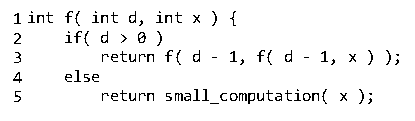
\includegraphics{just_calling_benchmark}
\caption{The microbenchmark for measuring call frame allocation overhead.}
\label{fig:micro_calling}
\end{figure}

Most importantly all the calls in the first version of this test were performed in yielding mode.
In no-yield mode, calls and returns in \charcoal{} are just as efficient as plain C.
In well-tuned \charcoal{} code, most of the leaf and near-leaf calls should be performed in no-yield mode.
To simulate this effect, we modified the benchmark to the version in Figure \ref{fig:micro_calling_n}.
The parameter \texttt{N} controls how deep in the call tree the benchmark uses yielding mode, before switching to no-yield.

\vspace{1em}
\begin{tabular}{|l|r|r|r|}
  \hline
   & user & sys & wall \\
  \hline
  \hline
  Plain C & 0.77 & 0.00 & 0.77 \\
  \hline
  Hot Stacking, \texttt{N} = 4 & 11.0 & 0.01 & 11.0 \\
  \hline
  Hot Stacking, \texttt{N} = 8 & 1.54 & 0.00 & 1.55 \\
  \hline
\end{tabular}
\vspace{1em}

This shows that with a modest fraction of the (static) calls performed in no-yield mode, the calling overhead gets down to less than a factor of 2.
Combined with the observations above about tuning the language implementation and real application performance, we believe this overhead is tolerable for most applications.
Also it is worth noting that this is the price to be paid for the extremely low memory overhead of activities.

\begin{figure}
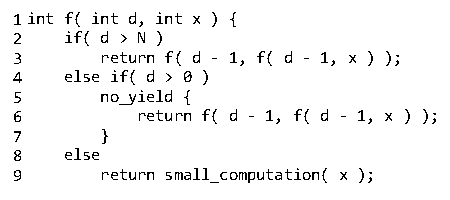
\includegraphics{just_calling_n_benchmark}
\caption{The call/return microbenchmark modified to make some calls in no-yield mode.}
\label{fig:micro_calling_n}
\end{figure}

\subsection{Yielding}

As described above, yielding is made fast by two tricks:
First, when code is executing in no-yield mode it simply does not yield at all.
Second, the fast common case for yielding is just performing an atomic read on a global variable and branching.
Even with this fast implementation, yielding is still not free.
It is important to completely avoid yielding in hot inner loops whenever possible.

To quantify this overhead, we benchmarked a simple but problematic function from the C standard library: \texttt{strcmp}.
\texttt{strcmp} is tricky for a few reasons:
First, the input strings could be very long, so it is not acceptable to make the implementation simply never yield.
Second, the body of the loop is extremely simple; good implementations are just a few assembly instructions.
This means that yielding every iteration would cause significant performance overhead.
Third, whether each iteration executes depends on the computation of the previous iteration, so simple loop tiling/blocking tricks do not work.
The best-performing implementation we have found so far appears in Figure \ref{fig:strcmp}.

\begin{figure}
    \centering
    \begin{subfigure}[b]{0.3\textwidth}
        \hspace{-1.5cm}
        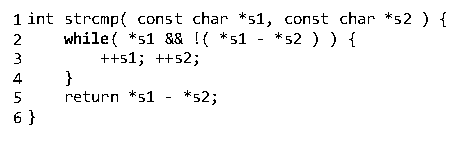
\includegraphics{plain_strcmp}
        \caption{}
    \end{subfigure}
    ~ %add desired spacing between images, e. g. ~, \quad, \qquad, \hfill etc. 
      %(or a blank line to force the subfigure onto a new line)
    \begin{subfigure}[b]{0.3\textwidth}
        \hspace{-1.5cm}
        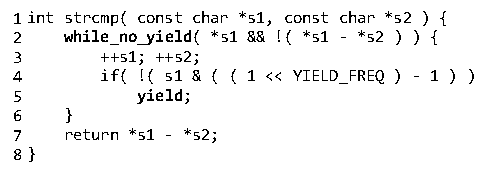
\includegraphics{strcmp_benchmark}
        \caption{}
    \end{subfigure}
    \caption{Two implementations of \texttt{strcmp}.
      (a) is a plain C version.
      (b) is a \charcoal{} implementation aimed at minimizing yield overhead. }
    \label{fig:strcmp}
\end{figure}

\texttt{while\_no\_yield} is a special variant of the regular while loop that does not have an implicit yield after every iteration.
This is different from wrapping a regular while loop in \texttt{no\_yield}, because the latter would prevent nested yields from happening, whereas the former does not.

In the code \texttt{YIELD\_FREQ} controls how frequently the loop yields.
The effect is that once every $2^{(\mathtt{YF})}$ iterations there is a yield.

\vspace{1em}
\begin{tabular}{|l|r|}
  \hline
  Plain C & 430 \\
  \hline
  \charcoal, \texttt{YIELD\_FREQ = 4} & 1070 \\
  \hline
  \charcoal, \texttt{YIELD\_FREQ = 8} & 519 \\
  \hline
  \charcoal, \texttt{YIELD\_FREQ = 12} & 446 \\
  \hline
\end{tabular}
\vspace{1em}

These numbers are in microseconds per \texttt{strcmp} of two identical strings of 1MB length.
These data show that yielding is far from free, but with a little careful tuning the yield overhead can be brought quite low.
Recall that yield frequency can be as low as about once per millisecond without negatively affecting most applications, so yielding every 4000 iterations (as in the \texttt{YIELD\_FREQ = 12} case) is fine.

In cases where the calling code is certain that the parameter strings are reasonably short, it can simply call \texttt{strcmp} in no-yield mode.
In this case the performance should be identical to the plain C implementation.

% \subsection{Code Size}

\subsection{Microbenchmark Summary}

Like all well implemented coroutines/cooperative threads, the \charcoal{} implementation has extremely low memory and time overhead for basic concurrency primitives.
Hot stacking and frequent yielding are potential performance issues, but our tests indicate that at these overheads can be managed.

%% \section{Foreign Code}

%% Foreign code (including legacy code) will never yield.  This could lead
%% to starvation pretty easily.  Here are three strategies:

%% \begin{itemize}
%% \item Do nothing.
%%   Just run the foreign code.
%%   This is a perfectly reasonable strategy as long as the foreign code does not run for a long time.
%% \item Run the foreign code in its own thread.
%%   If it has not returned by the end of some time slice, pause it to allow other activities to run.
%%   This runs the risk of creating atomicity violations galore.
%%   It also reintroduces the possibility of data races.
%%   However, it might be a reasonable strategy in situations where there is very little sharing between the foreign code and the rest of the application.
%% \item Run the foreign code in its own thread, but only interrupt it at special ``safe-ish'' points, like system calls.
%%   This is a compromise between the previous two strategies in the sense that it opens the door to both starvation and atomicity violations, but provides some (imperfect) protection against both.
%% \end{itemize}

%% We have not thought at all about what the best default is or what syntactic sugar would be nice.

%% Another important implementation issue to consider is foreign code that calls back in to activity-aware code.
%% There will definitely be some fancy footwork necessary there, no matter which strategy is used.

\section{Related Work}

As mentioned in the introduction, there are many projects that have aimed for a hybrid somewhere between threads and events.
One of the closest to the system reported here is Continuation Passing C (CPC) \cite{Kerneis2013}.
In that work the authors focus on the ability to switch back and forth between preemptive and cooperative modes, rather than a single abstraction that combines the best of both.
In some of the CPC publications, the designers claimed that it was not possible to implement some more exotic features of C, like setjmp/longjmp and alloca.
A detailed description of our implementation of these features is beyond the scope of this paper, but a working implementation is available in the project repository.
The hot stacking frame allocation strategy makes the implementation of these features (and related things like exceptions) more complicated, but not impossible.

One weakness that activities share with most multitasking frameworks is that activities cannot easily be run in parallel.
Naively running activities simultaneously on parallel processors would immediately violate the simple sequential memory model.
However, it is interesting to consider what it would take to run activities in parallel without violating their semantics.
The most obvious way to accomplish that would be with a transactional memory system; every activity would always be running in a transaction.
Yielding would cause one transaction to end and the next to begin.
The authors are not optimistic that such a transaction based system would work well, but other researchers are pursuing this kind of idea \cite{ONeill2015, Boussinot2006, Dabrowski2006}.

Our opinion is that parallelism should be accomplished with isolated processes.
Units of work can be dispatched to multitasking primitives (like events, coroutines or activities) running in isolated worker processes.
This is not a simple software architecture, but it does provide processor parallelism while largely avoiding the nasty mess of shared memory parallelism.

%% Threads are the only multitasking abstractions discussed in this paper that naturally allow the parallel execution of tasks.
%% The authors view this as closer to a bug than a feature.
%% Serial multitasking abstractions like events and coroutines (and activities) can be used in combination with parallelism frameworks like processes and threads.
%% The authors consider providing both parallelism and multitasking in a single language features (like threads) mostly a bad idea.
%% Nevertheless, in the discussion section at the end of this paper we speculate about the feasibility of running activities in parallel.


% Threads without the Pain

\subsection{Other Multitasking Abstractions}

There multitasking abstractions that we did not analyze earlier in the paper.
We mention them briefly here, only to argue that they are more distantly related for one reason or another.

\textbf{Isolated processes}.
Isolated process can be used for multitasking.
However, for things like handling GUI events, database transactions and network communication, shared memory is an extremely useful feature.

\textbf{Functional reactive programming}.
Functional reactive programming (FRP) is an entirely different approach to multitasking.
The central idea is that observable outputs are pure functions (potentially very complicated ones) of live inputs.
This is an interesting idea, but it is not clear whether it can be implemented efficiently and integrated with mainstream programming practice.



\section{Summary and Discussion}

In this paper we introduced pseudo-preemptive threads/activities, a new multitasking primitive.
Activities have advantages in reliability, composability and/or maintainability over the most common approaches to writing multitasking software (events, threads and coroutines).
From an application programmer's perspective activities feel most like threads, but they do not suffer from several of the nasty concurrency problems that plague multithreaded software.
Activities also have extremely low memory and time overheads compared to conventional thread implementations.
Activities can be thought of as actually working the way inexperienced programmers think threads should work, which we think is a good thing.

% \acks

% Acknowledgments, if needed.

% We recommend abbrvnat bibliography style.

\bibliographystyle{abbrvnat}

% The bibliography should be embedded for final submission.

\bibliography{../../../../Documents/PapersForReferencing/biy_all_research.bib}

%% \begin{thebibliography}{../../../../Documents/PapersForReferencing/biy_all_research.bib}
%% \softraggedright

%% \end{thebibliography}

\end{document}
